\subsection{Rail-Editor}

\begin{frame}{Rail-Editor}

\begin{figure}
  \begin{center}
    \leavevmode
      \includegraphics[width = .75\textwidth]{editor}
    \caption{Team Rail-Editor}
  \end{center}
\end{figure}

\end{frame}

\begin{frame}{Rail-Editor}
	Übersicht:
	\begin{itemize}
		\pause
		\item Softwaretechnik
		\item Technische Aspekte
		\item Live-Demo
	\end{itemize}
\end{frame}

\begin{frame}{Rail-Editor: Softwaretechnik}
	\pause
	\begin{itemize}
	\item Kleines Team $\rightarrow$ Kommunikation per Email
	\pause
	\item Direkte Reaktionen auf Emails (an alle geschickt)
	\pause
	\item Zuerst zwei, ab dem 2. Meilenstein drei Mitglieder
	\begin{itemize}
	\item Bessere Arbeitsverteilung
	\end{itemize}
	\pause
	\item Zwei Daily Scrums pro Woche
	\pause
	\item Zusätzliche Team-Meetings in der Woche
	\begin{itemize}
	\item Produktives Arbeiten durch Pair-Programming
	\end{itemize}
	\pause
	\item Gute Kommunikation innerhalb des Teams
	\pause
	\item Anfangs spärliche Kommunikation mit den anderen Teams, am Ende wesentlich besser
	\end{itemize}
\end{frame}

\begin{frame}{Rail-Editor: Technische Aspekte I}
	\pause
	\begin{itemize}
		\item \textit{Qt} für Programmierung der grafischen Benutzeroberfläche
		\pause
		\item Signal- und Slottechnik
		\pause
		\item Eventverarbeitung für Maus- und Tastendrücke
		\pause
		\item Basisklassen abgeleitet und Funktionalitäten erweitert
		\pause
		\item Graphstruktur für Syntax-Highlighting
		\begin{itemize}
			\item Internes Backend
		\end{itemize}
	\end{itemize}
	
	\begin{figure}
		\centering
		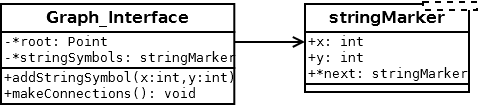
\includegraphics[width=0.7\textwidth]{syntax-highlighting}
	\end{figure}
\end{frame}

\begin{frame}{Rail-Editor: Technische Aspekte II}
	\pause
	\begin{itemize}
	\item Smart-Cursor und Grab-Modus
	\begin{itemize}
	\item Für intuitives Schreiben von Quellcode
	\item Siehe Live-Demo
	\end{itemize}
	\pause
	\item Main-Window als \textit{Anker}
	\begin{itemize}
	\item Weiterleitung an Child-Widgets
	\end{itemize}
	\pause
	\item Undo-Redo-Funktionalität
	\begin{itemize}
	\item Abstrakte Klasse
	\item Wird durch konkrete Aktionen implementiert
	\end{itemize}
	\pause
	\item Compiler-Einbindung
	\begin{itemize}
	\item Funktionen: Build, Run, Stop
	\item Der Rail-Interpreter kann ebenfalls verwendet werden
	\end{itemize}
	\pause
	\item \textit{Preferences} (Editor-Einstellungen)
	\begin{itemize}
	\item Persistente Speicherung
	\end{itemize}
	\end{itemize}
\end{frame}	

\begin{frame}{Rail-Editor: UML-Diagramm}	
	\begin{figure}
		\centering
		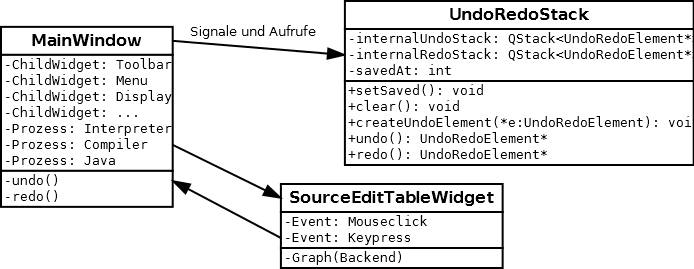
\includegraphics[width=0.9\textwidth]{editor-uebersicht}
	\end{figure}
\end{frame}

\begin{frame}{Rail-Editor: Live Demo}
	\begin{itemize}
		\item Live Demo
	\end{itemize}
\end{frame}